
\index{giảm chiều dữ liệu -- dimensionality reduction}
\index{dimensionality reduction -- giảm chiều dữ liệu}
\index{lựa chọn đặc trưng -- feature selection}
\index{feature selection -- lựa chọn đặc trưng}
\index{trích chọn đặc trưng -- feature extraction}
\index{feature extraction -- trích chọn đặc trưng}

\chapter*{MỞ ĐẦU}
\markboth{Mở đầu}{}
\addcontentsline{toc}{chapter}{MỞ ĐẦU}
\label{part: dimred}

\section{Lý do chọn đề tài}

Với sự phát triển không ngừng của khoa học và công nghệ, đặc biệt là với những
chiếc điện thoại thông minh (smartphone) ngày càng hiện đại và được sử dụng
phổ biến trong đời sống con người đã làm cho lượng thông tin thu được bằng hình ảnh
ngày càng tăng. Theo đó, lĩnh vực xử lý ảnh cũng được chú trọng phát triển, ứng dụng
rộng rãi trong đời sống xã hội hiện đại. Không chỉ dừng lại ở việc chỉnh sửa, tăng
chất lượng hình ảnh mà với công nghệ xử lý ảnh hiện nay chúng ta có thể giải quyết
các bài toán nhận dạng chữ viết, nhận dạng dấu vân tay, nhận dạng khuôn mặt...
Một trong những bài toán được nhiều người quan tâm nhất của lĩnh vực xử lý ảnh hiện nay
đó là nhận dạng khuôn mặt (Face Recognition). Như chúng ta đã biết, khuôn mặt đóng
vai trò quan trọng trong quá trình giao tiếp giữa người với người, nó mang một lượng
thông tin giàu có, chẳng hạn như từ khuôn mặt chúng ta có thể xác định giới tính, tuổi tác,
chủng tộc, trạng thái cảm xúc, đặc biệt là xác định mối quan hệ với đối tượng (có quen biết
hay không).

Có rất nhiều phương pháp nhận dạng khuôn mặt để nâng cao hiệu suất tuy nhiên dù ít hay
nhiều những phương pháp này đang vấp phải những thử thách về độ sáng, hướng nghiêng,
kích thước ảnh, hay ảnh hưởng của tham số môi trường. Bài toán
Nhận diện khuôn mặt (Face Recognition) bao gồm nhiều bài toán khác nhau như:
phát hiện mặt người (face detection), đánh dấu (facial landmarking), trích chọn(rút) đặc trưng
(feature extration), gán nhãn, phân lớp (classification).
Trong thực tế, nhận dạng khuôn mặt người (Face Recognition) là một hướng nghiên cứu được
nhiều nhà khoa học quan tâm, nghiên cứu để ứng dụng trong thực tiễn.
Vì thế có những cải tiến nghiên cứu về bài toán phát hiện khuôn mặt người trong
những môi trường phức tạp hơn, có nhiều khuôn mặt người trong ảnh hơn,
và có nhiều tư thế thay đổi trong ảnh... Trong bài này tôi sẽ tìm hiểu về trích rút đặc
trưng sử dụng học sâu (Deep learning) và áp dụng vào bài toán nhận diện khuôn mặt .

% Chúng ta sẽ xem xét các phương pháp giảm chiều dữ liệu phổ biến
% nhất: \textit{phân tích thành phần chính} ({principle component analysis}) cho bài toán giảm chiều dữ liệu
% vẫn giữ tối đa lượng thông tin, và \textit{linear discriminant analysis}
% cho bài toán giữ lại những đặc trưng quan trọng nhất cho việc phân loại. Trước
% hết, chúng ta cùng tìm hiểu một phương pháp phân tích ma trận vô
% cùng quan trọng  --  \textit{phân tích giá trị suy biến} ({singular value decomposition}).

\section{Mục đích của đề tài}

\begin{itemize}
      \item Xây dựng, tìm kiếm các mô hình học sâu để trích xuất thông tin khuôn mặt
            người dùng 1 cách chính xác, hiệu quả.
      \item Tìm hiểu sử dụng thành thạo các phương pháp làm giàu dữ liệu,
            ứng dụng cho bài toán nhận diện với dữ liệu là các ảnh khuôn mặt
      \item Xây dựng các phương pháp thu thập, làm giàu dữ liệu khuôn mặt
      \item Tìm hiểu ứng dụng các thuật toán phân loại trong học máy để
            áp dụng vào bài toàn nhận diện khuôn mặt
\end{itemize}

\section{Đối tượng và phạm vi nghiên cứu của đề tài}
\subsection{Đối tượng}
\begin{itemize}
      \item Các mô hình học sâu nổi tiếng về nhận dạng khuôn mặt được các nhà khoa học huấn luyện trước với nhưng bộ dữ liệu
            cực lớn và chuẩn xác.
      \item Các mô hình, phương pháp phát hiện khuôn mặt trong ảnh với độ chính xác cao
      \item Các phương pháp làm giàu dữ liệu, đặc biệt là với dữ liệu khuôn mặt.
      \item Các phương pháp phân loại dữ liệu trong học máy và học sâu
      \item Các phương pháp đánh giá mất mát thương dùng để huấn luyện các mô hình học máy, học sâu
\end{itemize}
\newpage
\subsection{Phạm vi nghiên cứu}
\begin{itemize}
      \item Tập trung sử dụng bộ dữ liệu tự tạo của các sinh viên trong trường đại học Công nghiệp Hà Nội
      \item Huấn luyện mô hình theo phương pháp đánh giá bộ ba (triplet loss)
      \item Sử dụng các đánh giá cơ bản để đánh giá tính chính xác của mô hình
\end{itemize}
\section{Kết cấu của đồ án}
Gồm 4 chương:

Chương 1: Nghiên cứu tổng quan

Chương 2: Cơ sở lý thuyết

Chương 3: Thiết kế và xây dựng hệ thống

Chương 4: Kết luận và hướng phát triển




%!TEX root = ../book_ML.tex

\def\R{\mathbb{R}}
\newpage
\section{Bảng các ký hiệu}
Các ký hiệu sử dụng trong sách được liệt kê trong Bảng~\ref{tab:notation}.

\begin{table}[h]
    \caption{Các quy ước ký hiệu và tên gọi được sử dụng trong báo cáo}
    \label{tab:notation}
    \centering
    \begin{tabular}{|c|l|}
    \hline 
    Ký hiệu & Ý nghĩa  \\ \hline 
    \hline 
    $x, y, N, k$ & in nghiêng, thường hoặc hoa, là các số vô hướng \\ \hline
    $\bx, \by$ & in đậm, chữ thường, là các vector  \\ \hline
    $\bX, \bY$ & in đậm, chữ hoa, là các ma trận  \\ \hline
    $\R$ & tập hợp các số thực \\ \hline 
    $\mathbb{N}$ & tập hợp các số tự nhiên \\ \hline 
    $\mathbb{C}$ & tập hợp các số phức \\ \hline 
    $\R^{m}$ & tập hợp các vector thực có $m$ phần tử \\ \hline 
    $\R^{m\times n}$ &tập hợp các ma trận thực có $m$ hàng, $n$ cột \\ \hline
    $\mathbb{S}^n$ & tập hợp các ma trận vuông đối xứng bậc $n$ \\ \hline 
    $\mathbb{S}^n_{+}$ & tập hợp các ma trận nửa xác định dương bậc $n$ \\
    \hline 
    $\mathbb{S}^n_{++}$ & tập hợp các ma trận xác định dương bậc $n$ \\ \hline 
    $ \in $ & phần tử thuộc tập hợp \\ \hline 
    $ \exists $ & tồn tại \\ \hline 
    $ \forall $ & mọi \\ \hline 
    $ \triangleq$ & ký hiệu là/bởi. Ví dụ $a\triangleq f(x)$ nghĩa là ``ký hiệu
    $f(x)$ bởi $a$''. \\ \hline 
    $x_i$ & phần tử thứ $i$ (tính từ 1) của vector $\bx$ \\ \hline 
    $\sgn(x)$ & hàm xác định dấu. Bằng 1 nếu $x \geq 0$, bằng -1 nếu $x < 0$. \\ \hline
    $\exp(x)$ & $e^x$ \\ \hline
    $\log(x)$ & logarit \textit{tự nhiên} của số thực dương $x$ \\ \hline
    $\displaystyle \argmin_xf(x)$ & giá trị của $x$ để hàm $f(x)$ đạt giá trị nhỏ nhất \\ \hline 
    $\displaystyle \argmax_xf(x)$ & giá trị của $x$ để hàm $f(x)$ đạt giá trị lớn nhất \\ \hline 
    % $a_{ij}$ & phần tử hàng thứ $i$, cột thứ $j$ của ma trận $\bA$ \\ \hline 
    % $\bA^T$ & chuyển vị của ma trận $\bA$ \\ \hline 
    % $\bA^H$ & chuyển vị liên hợp (Hermitian) của ma trận phức $\bA$ \\ \hline 
    % $\bA^{-1}$ & nghịch đảo của ma trận vuông $\bA$, nếu tồn tại \\ \hline 
    % $\bA^{\dagger}$ & giả nghịch đảo của ma trận không nhất thiết vuông $\bA$ \\
    % \hline 
    % $\bA^{-T}$ & chuyển vị của nghịch đảo của ma trận $\bA$, nếu tồn tại \\ \hline 
    % $\|\bx\|_p$ & $\ell_p$ norm của vector $\bx$ \\ \hline  
    % $\|\bA\|_F$ &  Frobenius norm của ma trận $\bA$ \\ \hline 
    % $ \diag(\bA)$ & đường chéo chính của ma trận $\bA$ \\ \hline 
    % $\trace(\bA)$ & trace của ma trận $\bA$ \\ \hline 
    % $\det(\bA)$ & định thức của ma trận vuông $\bA$ \\ \hline 
    % $\text{rank}(\bA)$ & hạng của ma trận $\bA$ \\ \hline 
    o.w & \textit{otherwise}  --  trong các trường hợp còn lại \\ \hline 
    $\displaystyle\frac{\partial f}{\partial x}$ & đạo hàm của hàm số $f$ theo $x \in \R$ \\ \hline
    $\nabla_{\bx}f$ & gradient của hàm số $f$ theo $\bx$ ($\bx$ là vector hoặc ma trận) \\ \hline 
    $\nabla^2_{\bx}f$ & gradient bậc hai của hàm số $f$ theo $\bx$, còn được gọi là \textit{Hesse} \\ \hline 
    $\odot$ & \makecell{Hadamard product (elemenwise product). Phép nhân từng phần tử \\ của hai vector hoặc ma trận cùng kích thước.} \\ \hline 
    $\propto$ & tỉ lệ với \\ \hline 
    % v.v. & vân vân \\ \hline 
    %%%%%%%
    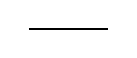
\begin{tikzpicture}
    \draw [thick] (0, 0) -- (1, 0); 
    \end{tikzpicture}
    & đường nét liền \\ \hline 

    %%%%%%%
    \begin{tikzpicture}
    \draw [very thick, dashed] (0, 0) -- (1, 0); 
    \end{tikzpicture}
    & đường nét đứt \\ \hline 

    %%%%%%%
    \begin{tikzpicture}
    \draw [very thick, dotted] (0, 0) -- (1, 0); 
    \end{tikzpicture}
    & đường nét chấm (đường chấm chấm)\\ \hline 

    %%%%%%%
    \begin{tikzpicture}
    \draw [very thick, dash pattern={on 7pt off 2pt on 1pt off 3pt}] (0,0) -- (1,0);
    \end{tikzpicture}
    & đường chấm gạch\\ \hline 
    %%%%%%%
    % \\[-3mm]
    % \vspace{1em}
    \begin{tikzpicture}[yshift = -1cm]
    \draw [pattern = dots] (0,0) rectangle (1,.4);
    \end{tikzpicture}
    & nền chấm\\\hline 
    %%%%%%%
    % \\[-1em]
    % \vspace{1em}
    \begin{tikzpicture}
    \draw [pattern = custom north west lines] (0,0) rectangle (1,.4);
    \end{tikzpicture}
    & nền sọc chéo\\ \hline 



    \end{tabular}
 \end{table} 
